\documentclass[10pt]{article}
\usepackage[margin=18mm]{geometry}
\usepackage{graphicx,booktabs,hyperref}
\usepackage[strings]{underscore}
\setlength{\parindent}{0pt}\setlength{\parskip}{5pt}
\begin{document}
\section*{Narrow quartic constructor: preserved field, fewer recorded instructions}

Original runs 2026-10-25; native provenance/accounting audit 2026-10-26.
Baseline source 335d168aac85, binary SHA prefix 81ab248653df; candidate library
source c754e7111. Same narrow6 workload, one thread, shared AMD EPYC 9V74
Linux x86-64 host, L0. Raw manifests and both executable hashes are checked.

\begin{center}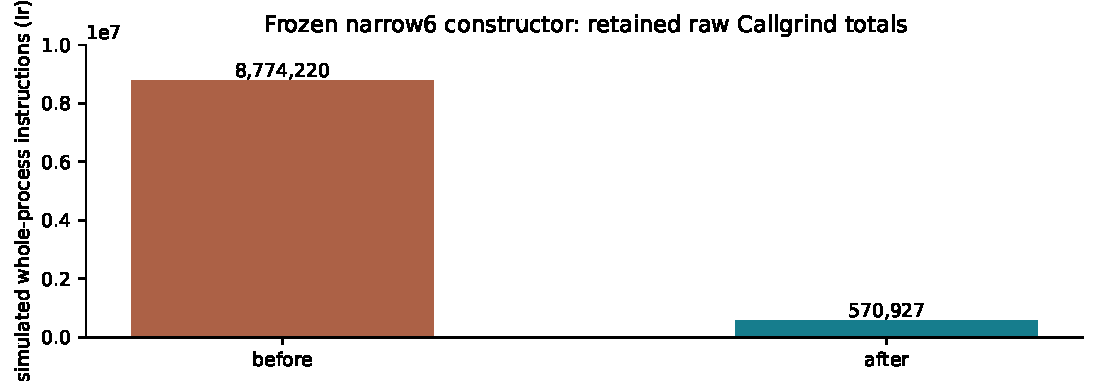
\includegraphics[width=.92\linewidth]{narrow-constructor-instructions.pdf}\end{center}
The simulated whole-process totals are 8,774,220 and 570,927 Ir. They include
loader/startup work and the Valgrind allocator. Complete stdout is
byte-identical. All seven frozen m=4--10 even/odd controls return identical
base polynomials, quartic coefficients and checked field products. The
library gate on this source passed 4,635 tests, zero failed, 119 ignored;
affected example tests and scoped clippy pass. These are recorded source
checks, not checks on a later merged PR head.

The change excludes c3=0 for even m and c3=c1=0 for every m, preserving
the first irreducible field. The readable exclusion and six checked Lean
algebraic dependencies are retained; finite-field specialization and the
irreducibility bridge remain unformalized. Original active quartic runs used
their separate frozen binary and were not modified by this change.

\textbf{Limits.} This is instruction attribution, not native runtime,
physical throughput, a fastest-external-tool comparison, or a complete-IC
speedup. Repeated A/A and interleaved native A/B controls, complete phase
prices and matched whole-pipeline comparisons remain missing. No new
leaderboard or admitted benchmark row follows.

\begin{flushleft}\footnotesize
Native source: examples/ic_followup_publication_audit.rs.\par
Receipt: \texttt{../../pipeline-receipts/publication-followup-audit-v3-20261026/output.json}.\par
Protocol: NARROW_CONSTRUCTOR_EXCLUSION_PROTOCOL.md and FOLLOWUP_PUBLICATION_AUDIT_PROTOCOL.md.\par
Archive: evidence/runs-narrow-constructor-checked-20261026.tar.xz.\par
Existing PDFs and raw measurements are unchanged; new oversized artifacts remain local pending verified store upload.
\end{flushleft}

\end{document}
